\section{Auswertung}
\label{sec:Auswertung}

In \autoref{fig:auge} sind die Ergebnisse der Untersuchung des Augenmodells mit einem A-Scan mit Impuls-Echo-Verfahren zu sehen.
\begin{figure}[H]
  \centering
  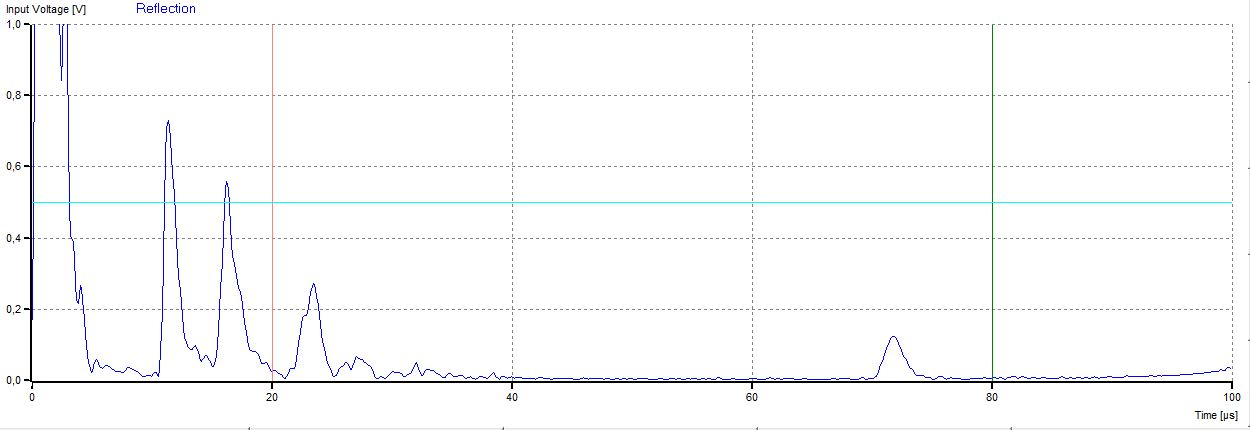
\includegraphics[width=\textwidth]{messungen/auge/auge.jpg}
  \caption{Spannungs-Zeit Diagramm zum A-Scan des Augenmodells}
  \label{fig:auge}
\end{figure}

\cite{sample}
Die ersten beiden in \autoref{fig:auge} zu sehenden Peaks werden als der Ein- und Austritt des Ultraschalls in die bzw. aus der Linse interpretiert. Der dritte Peak entspricht dem Echo des Ultraschalls von der Rückwand der Retina. Mit den bekannten Schallgeschwindigkeiten für die Linse ($c_{L} = 2500 m/s$) und die Glaskörperflüssigkeit ($c_{GK} = 1410 m/s$) sowie den Daten des A-Scans lassen sich die Abmessungen des Augenmodells berechnen. Aus den Messdaten konnten die Zeiten der 3 Peaks ermittelt werden:\newline
1.Peak: $11,4 \mu s$ \newline 2.Peak: $16,3 \mu s$ \newline 3.Peak: $23,2 \mu s$ \newline
Mit ergeben sich für die Maße des Augenmodells:
\begin{table}
  \centering
  \caption{Abmessungen des Augenmodells}
\label{tab:mess2}
  \sisetup{table-format=2.1}
  \begin{tabular}{c c c c}
  \toprule
  Strecke & Zeit $[\mu s]$ & Weg[$mm$]\\
  \midrule
  Hornhaut-Linse & 11,4 & 8,037 \\
  Innerhalb der Linse & 4,9 & 6,125\\
  Linse-Retina & 6,9 & 4,865\\
  \bottomrule
  \end{tabular}
  \end{table}